\section{Parallel strategy} 
We begin by assigning the original complex array
$A(0:N_x-1,0:N_y-1,0:N_z-1)$ of data size $N_x \times N_y \times N_z$
in a block distribution onto a $P_x \times P_y \times P_z$
grid of nodes.  Thus, each node has a local array
$A'(0:n_x-1,0:n_y-1,0:n_z-1)$ of size $n_x \times n_y \times n_z$ where
$n_x = \frac{N_x}{P_x},n_y = \frac{N_y}{P_y}, n_z = \frac{N_z}{P_z}$.
 
If we denote by $A'(i,j,k)[x,y,z]$ the element $(i,j,k)$ of local
array $A'$ in the node at mesh coordinates $(x,y,z)$, then

\begin{figure}
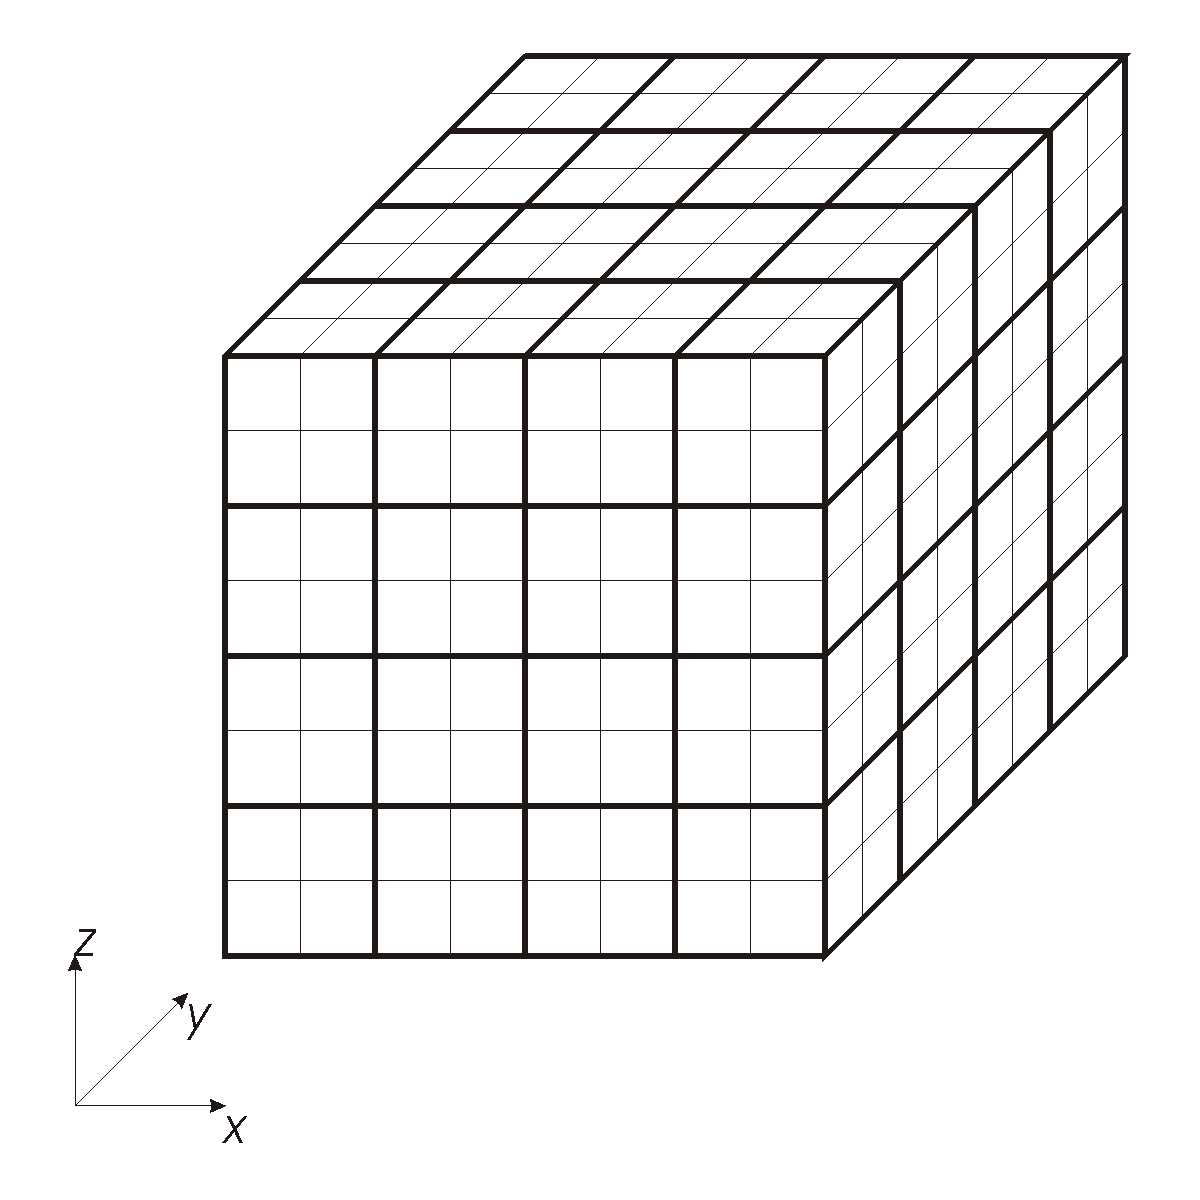
\includegraphics[keepaspectratio,width=\columnwidth]{fft_mesh_1}
\caption{Data distribution (light lines) and processor mesh (heavy
  lines) for an $\mathbf{8\times 8\times 8}$ FFT on a $\mathbf{4\times 4\times4}$
  processor mesh.}
\label{fig:domain_decomp}
\end{figure}

\begin{equation}
A'(i,j,k)[x,y,z] \equiv A(x n_x+i,y n_y+j,z n_z+k).
\end{equation}
Figure~\ref{fig:domain_decomp} shows the original data
distribution,(i.e. how the data is distributed among all the
processors) before any communication takes place.

For clarity, we impose the following restrictions on the sizes of the
local array $A'$: $n_x * n_y = \alpha \times P_z$, $n_y *n_z = \beta
\times P_y$, and $n_y * n_z = \gamma \times P_x$, where $\alpha$,
$\beta$, and $\gamma$ are integers.

We use the row-column approach described in the previous publication
to compute the 3D-FFT. That is, we first compute $N_x \times N_y $
1D-FFT along the z axis. Followed by $N_x \times N_z$ 1D-FFT in the y
axis and finally, $N_y \times N_z$ 1D-FFTs in the x axis.  This
requires successive transpositions of the global array.

Since the $N_x \times N_y$ one-dimensional FFTs along the $z$
dimension are all independent, we need only consider a single
processor row in the z dimension, which has to compute $n_x \times
n_y$ one-dimensional FFTs of size $N_z$. Let $A(0:n_x-1, 0:n_y-1,
0:N_z-1)$ block distributed along the z dimension. Then the local
array $A'(0:n_x-1, 0:n_y-1, 0:n_z-1)$ one node p in the original
decomposition is given by
 
\begin{eqnarray}
&A'_z(i,j,k)[p] \equiv A_z(i,j ,p \times  n_z+k)\\
\end{eqnarray}

Then we redistribute the data along both the $x$ and $y$ dimensions
onto the $P_z$ nodes. Let us assume that the number of 1D-FFTs to be
computed along the z dimension is smaller than the processor mesh
dimension $P_z$ (ie $\alpha=0$).  Then only those processors, p, along the z
axis that satisfy the condition $p \pmod {S_z} = 0$ with $S_z
(=\frac{P_z}{n_x n_y })$ compute a 1D-FFT along the z dimension. If
$A''(0:0,0:0, 0:Nz-1)$ array is the local array in node $p$ then,
\begin{eqnarray}
&A''_z(i,j,k)[p] \equiv A_z(i+\frac{ (p/S_z) }{n_y},j+(p/S_z)\pmod{n_y},k),\\
&if \{ p\pmod{S_z}=0 \}, \\
&A''_z(i,j,k)[p]=0,\\
&if \{ p\pmod{S_z}\ne 0\}, 
\end{eqnarray}
 
This new distribution of array A is shown in Fig 2. Once the data is
in this new form each node performs one 1D-FFT.

We expect this approach to have better performance than the one where
the 1D-FFTs are computed only on dense subset of nodes in the center
of the partition as shown in Figure~\ref{fig:dense}.  In the current
approach, with nodes computing 1D-FFTs spread evenly throughout the
partition, we expect reduced link contention.
